\section{Case Study}

\noindent
In this section we describe a realistic application of the system studied in this paper to perform surveillance operations. Considering the current COVID-19 restrictions, we focus on the problem of preventing and identifying possible concentrations of people during events such as popular or religious festivals. In particular we consider the Courtyards Festival of Cordoba (\url{https://patios.cordoba.es/es/}). This is a social event that takes place every year in the city of Cordoba, Spain, during the first two weeks of May. Courtyard’s owners decorate their houses with many flowers trying to win the award that is offered by the Town Hall. During this competition a festival runs in parallel with a number of artistic performances along six different paths located in different areas in the city as shown in Figure \ref{fig:mapPF}.
In the pandemic context, to monitor the situation to avoid concentration of people, we propose to apply a system consisting of one helicopter and a fleet of three drones.
This kind of system has been proved successfully and has been already applied in the military field by the US Army in order to leave the helicopter to the edge of dangerous airspace and release drones, which will then penetrate enemy territory and send back intelligence, surveillance and reconnaissance information (see \cite{FG}).
In our application the reason to adopt a similar system is the possibility to inspect simultaneously and in real time different paths also reducing the risk of flying the helicopter over populated areas and the cost for moving the helicopter by minimizing the total length of its tour.

\begin{figure}[h!]
\centering
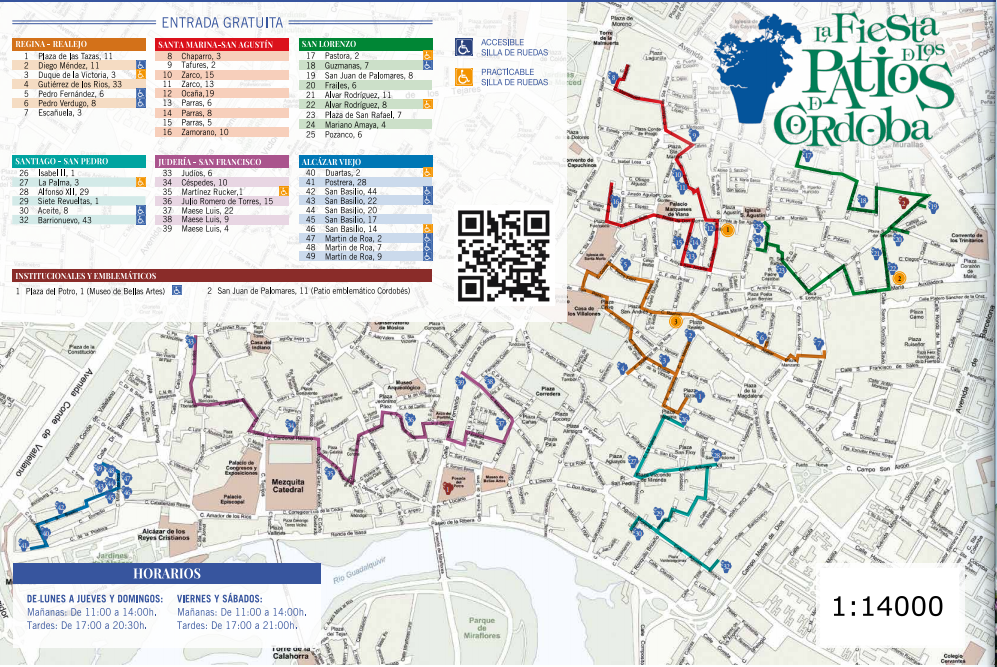
\includegraphics[width=0.6\linewidth]{figures/first.png}
\caption{Map of the Courtyards Festival in Cordoba. \label{fig:mapPF}}
\end{figure}

\noindent
We run the model presented in Section \ref{Form} on this scenario starting from the initial solution provided by the matheuristic, where the 6 coloured paths reported in the map of Figure \ref{fig:mapPF} represent the 6 target graphs to be visited, in this case inspected, by the fleet of drones. In addition, we suppose that the drones' speed is 100 km/h while that of the helicopter is  50 km/h aiming to minimize costs.
Moreover, we assume that the fleet is composed by three drones with an endurance equal to 2 hours, and we impose that each target graph must be fully visited (inspected).  As we can see from Figure \ref{fig:Mtour}, the origin of the mothership tour coincides with the destination and it is located in an area of the city where it is possible to assume the take-off and landing of an helicopter. Figure \ref{fig:Mtour} reports the tour followed by the helicopter in the solution obtained within the time limit of 2 hours sets to solve the model and with a percentage gap equal to 83\%. We can observe that the helicopter, starting from the origin, flies to the point $x_L^1$ that is the first launching point and then flies along the edge connecting $x_L^1$ with $x_R^1$, that is the first rendezvous point. Next, the helicopter flies to $x_L^2$ for launching the second drones' mission that are retrieved at point $x_R^2$. The third and last mission starts from $x_L^3$ and ends at point $x_R^3$ from where the helicopter goes back to the final destination.\\
Figure \ref{fig:tourD} shows the tour followed by the three drones for inspecting the six paths. In particular, one drone, in red, starts from $x_L^1$ for visiting the path of "Alcazar Viejo". From the same point a second drone, in green, starts for visiting the path of "Santa Maria-San Agustin". Both drones end their first mission at point $x_R^1$, where they are retrieved by the helicopter. Then, the helicopter flies to point $x_L^2$ where only one drone, the red one, starts its second mission to visit the path of "Juderia-San Francisco". In the meanwhile the helicopter, containing the other two drones, flies to point $x_R^2$ where it retrieves the previously launched drone. The last mission involves all the three drones that are launched from point $x_L^3$. The first drone, the red one, visits the path of "San Lorenzo", the second, the green one, visits the path of "Regina-Realejo" and the third, the blue one, visits the path of "Santiago-San Pedro".
All the three drones are retrieved by the helicopter at point $x_R^3$ and after that the helicopter goes back to the destination. 
The total distance travelled by the helicopter is equal to 11.27 km.

All details of this case study, including maps coordinates, .lp models and solutions can be found in \cite{Puerto2021}.


\begin{figure}[h!]
\centering
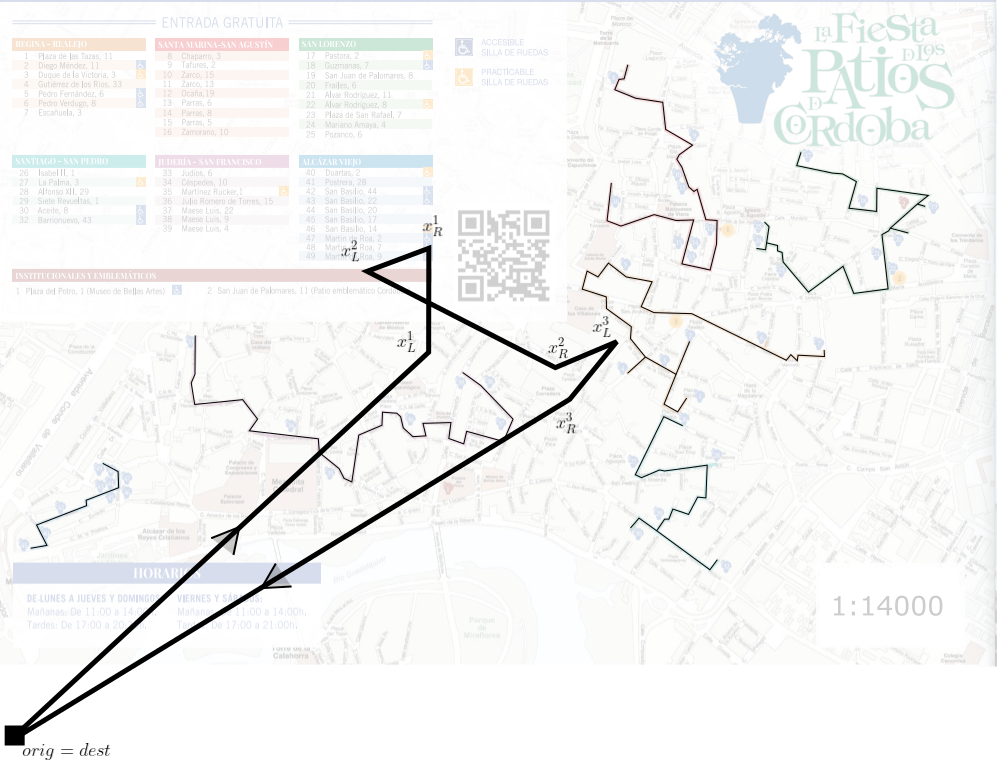
\includegraphics[width=0.6\linewidth]{figures/second.png}
\caption{Mothership tour. \label{fig:Mtour}}
\end{figure}

\begin{figure}[h!]
\centering
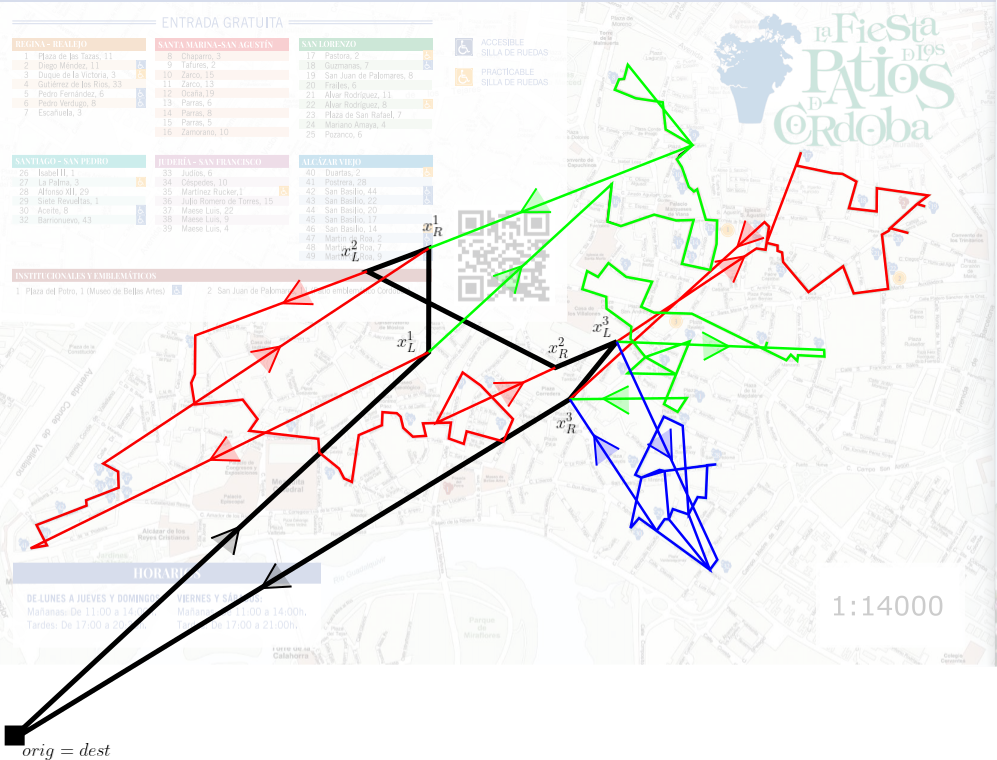
\includegraphics[width=0.6\linewidth]{figures/third.png}
\caption{The complete solution. \label{fig:tourD}}
\end{figure}